

\frame{
%\subsection{Parte I}
%\frametitle{Parte I. HMM per l'analisi della deambulazione: definizione}
\frametitle{Definizione di un'Hidden Markov Model (HMM)}
\begin{columns}
\column{.6\textwidth}

	\begin{figure}
	\centering
	  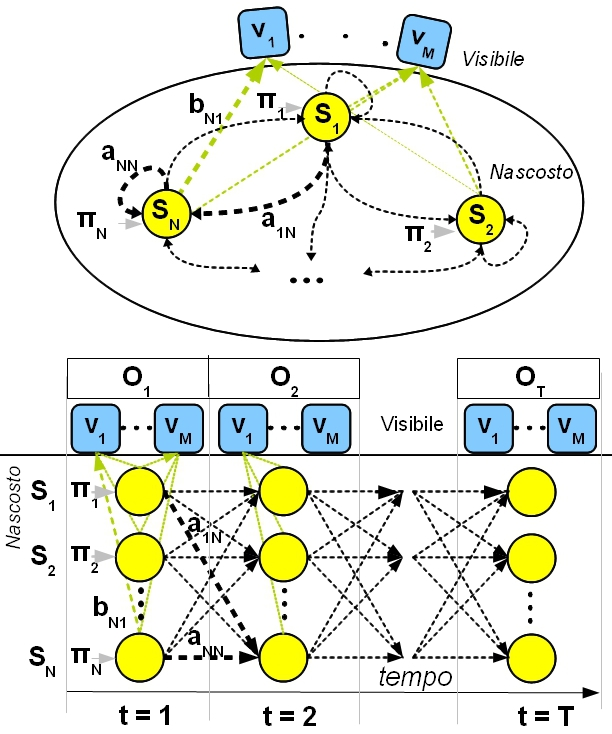
\includegraphics[width=.9\textwidth]{imgs/descreteMarkovProcesses2.jpg}	
	\end{figure}

\column{.5\textwidth}

%	\tiny{
	HMM $= <N, M, \mathbf{A}, \mathbf{B}, \mathbf{\pi}>$
dove: 

\begin{enumerate}
	\item $N = |S|$: stati nascosti
	\item $M = |V|$:  alfabeto osservazione
	\item $\mathbf{A}\{a_{ij}\}$: probabilit� di transizione 
				$a_{ij} = \wp[q_t = S_j | q_{t-1} = S_i]$
	\item $\mathbf{B}$ :probabilit� di emissione
				$b_j(k) = \wp[v_k \; \text{all'istante } t | q_t = s_j] $
	\item $\mathbf{\pi}$: probabilit� a priori
				$\pi_i = \wp(q_1 = S_i)$
				
\end{enumerate}

\end{columns}
%}

}



\frame{
%\subsection[Segmentazione]{Parte I. Segmentazione dei dati giroscopici relativi alla deambulazione}
\frametitle{La segmentazione: algoritmo di Viterbi}
%\begin{algorithm} 
%\caption{Viterbi}
%\label{alg:viterbi}                                                  
\begin{columns}
\column{.5\textwidth}
Viterbi
\begin{algorithmic}[1]                    
\STATE{}\COMMENT{\textit{Inizializzazione}}
\FOR {$i = 0$ to $N$}
	\STATE {$\delta_{i,1} = \pi_i b_i(o_1)$}
	\STATE {$\psi_{i,1} = 0$}
\ENDFOR
\STATE{}\COMMENT{\textit{Iterazione}}
\FOR{$t = 2$ to $T$}
	\FOR{$i = 1$ to $N$} 
		\STATE $ \delta_{i,t}=\displaystyle\max_{1\leq j \leq N} [\delta_{j,t-1}a_{j,i}]* b_i(o_i)$
		\STATE $ \psi_{i,t}=\displaystyle\arg \max_{1\leq j \leq N} [\delta_{j, t-1}a_{j,i}]$
	\ENDFOR
\ENDFOR
\STATE{}\COMMENT{\textit{Terminazione}}
\STATE $P* = \displaystyle \max_{1\leq i \leq N} [\delta_{i,T}]$
\STATE $q_T* = \displaystyle \arg \max_{1\leq i \leq N} [\delta_{i,T}]$
\STATE{}\COMMENT{Backtracking}
\FOR{$t=T-1$ to $1$}
	\STATE{$q*_t=\psi_{q*_{t+1},t+1}$}
\ENDFOR
\end{algorithmic}
%\end{algorithm}
\column{.5\textwidth}
\end{columns}
}